\documentclass{standalone}
\usepackage{tikz}
\usetikzlibrary{patterns, positioning}


\begin{document}
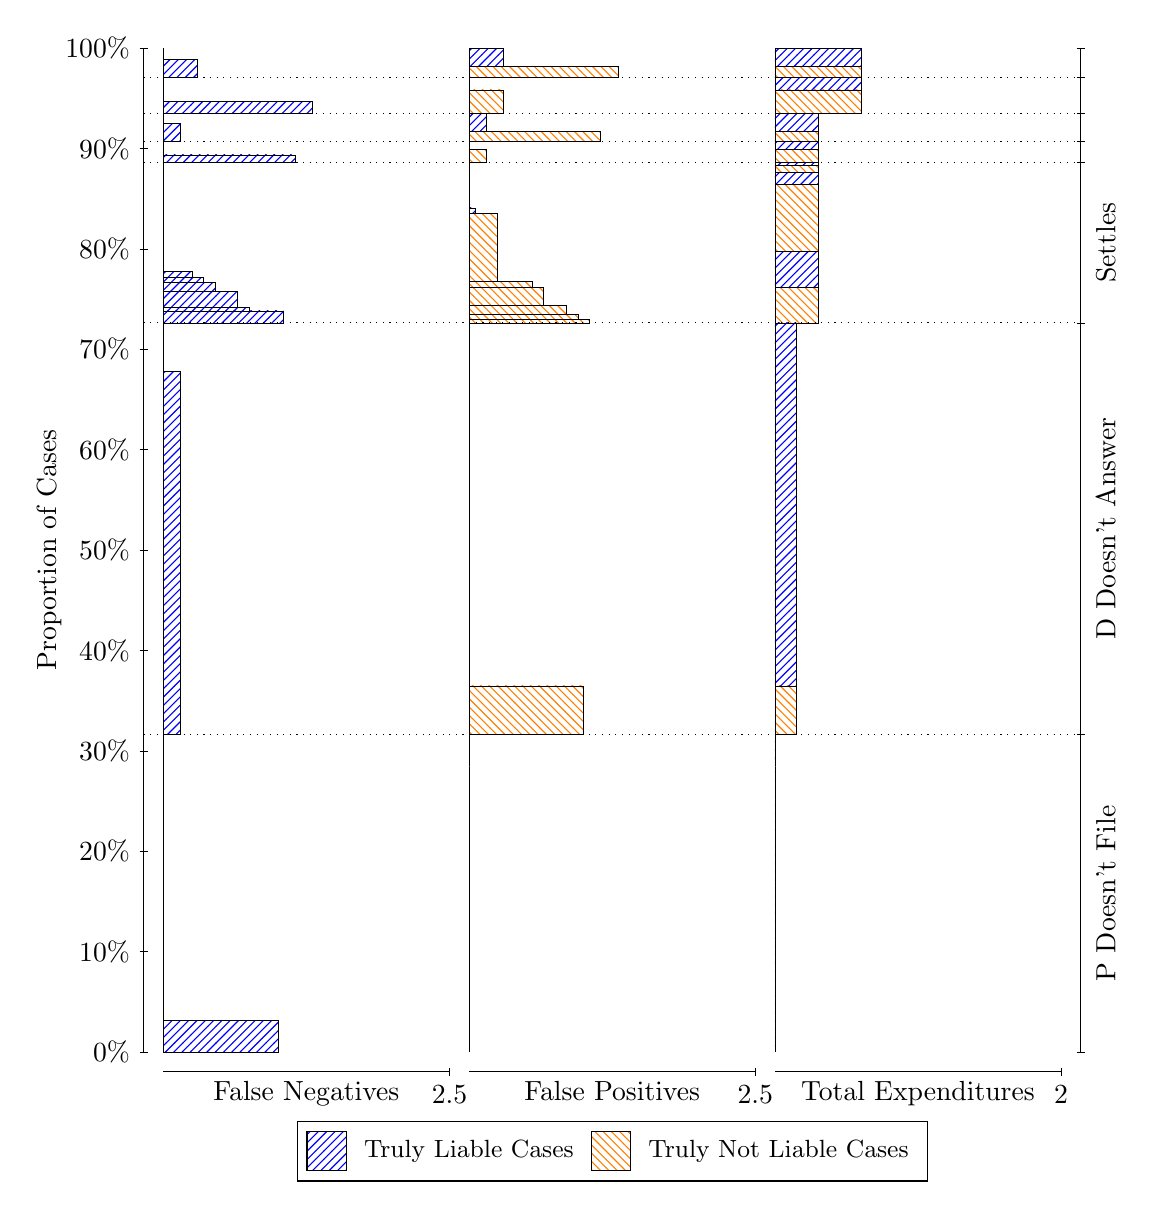
\begin{tikzpicture}
\draw[black, very thin] (1.5,1.75) -- (1.5,14.5);
\node[rotate=90, text=black, anchor=center] at (0.3, 8.125) {Proportion of Cases};
\draw[black, very thin] (1.45,1.75) -- (1.55,1.75);
\node[text=black, anchor=east] at (1.45, 1.75) {0\%};
\draw[black, very thin] (1.45,3.025) -- (1.55,3.025);
\node[text=black, anchor=east] at (1.45, 3.025) {10\%};
\draw[black, very thin] (1.45,4.3) -- (1.55,4.3);
\node[text=black, anchor=east] at (1.45, 4.3) {20\%};
\draw[black, very thin] (1.45,5.575) -- (1.55,5.575);
\node[text=black, anchor=east] at (1.45, 5.575) {30\%};
\draw[black, very thin] (1.45,6.85) -- (1.55,6.85);
\node[text=black, anchor=east] at (1.45, 6.85) {40\%};
\draw[black, very thin] (1.45,8.125) -- (1.55,8.125);
\node[text=black, anchor=east] at (1.45, 8.125) {50\%};
\draw[black, very thin] (1.45,9.4) -- (1.55,9.4);
\node[text=black, anchor=east] at (1.45, 9.4) {60\%};
\draw[black, very thin] (1.45,10.675) -- (1.55,10.675);
\node[text=black, anchor=east] at (1.45, 10.675) {70\%};
\draw[black, very thin] (1.45,11.95) -- (1.55,11.95);
\node[text=black, anchor=east] at (1.45, 11.95) {80\%};
\draw[black, very thin] (1.45,13.225) -- (1.55,13.225);
\node[text=black, anchor=east] at (1.45, 13.225) {90\%};
\draw[black, very thin] (1.45,14.5) -- (1.55,14.5);
\node[text=black, anchor=east] at (1.45, 14.5) {100\%};

\draw[black, very thin] (13.4,1.75) -- (13.4,14.5);
\draw[black, very thin] (13.35,1.75) -- (13.45,1.75);
\node[anchor=west] at (13.35, 1.75) {};
\draw[black, very thin] (13.35,5.7812) -- (13.45,5.7812);
\node[anchor=west] at (13.35, 5.7812) {};
\draw[black, very thin] (13.35,11.01) -- (13.45,11.01);
\node[anchor=west] at (13.35, 11.01) {};
\draw[black, very thin] (13.35,13.045) -- (13.45,13.045);
\node[anchor=west] at (13.35, 13.045) {};
\draw[black, very thin] (13.35,13.314) -- (13.45,13.314);
\node[anchor=west] at (13.35, 13.314) {};
\draw[black, very thin] (13.35,13.668) -- (13.45,13.668);
\node[anchor=west] at (13.35, 13.668) {};
\draw[black, very thin] (13.35,14.124) -- (13.45,14.124);
\node[anchor=west] at (13.35, 14.124) {};
\draw[black, very thin] (13.35,14.5) -- (13.45,14.5);
\node[anchor=west] at (13.35, 14.5) {};

\draw[black, very thin, pattern color=blue, pattern=north east lines] (1.75,1.75) rectangle (3.2033,2.1535);
\draw[black, very thin, pattern color=orange, pattern=north west lines] (1.75,2.1535) rectangle (1.75,5.7812);
\draw[black, very thin, pattern color=blue, pattern=north east lines] (1.75,5.7812) rectangle (1.968,10.393);
\draw[black, very thin, pattern color=orange, pattern=north west lines] (1.75,10.393) rectangle (1.75,11.01);
\draw[black, very thin, pattern color=blue, pattern=north east lines] (1.75,11.01) rectangle (3.276,11.163);
\draw[black, very thin, pattern color=blue, pattern=north east lines] (1.75,11.163) rectangle (2.84,11.203);
\draw[black, very thin, pattern color=blue, pattern=north east lines] (1.75,11.203) rectangle (2.6947,11.406);
\draw[black, very thin, pattern color=blue, pattern=north east lines] (1.75,11.406) rectangle (2.404,11.52);
\draw[black, very thin, pattern color=blue, pattern=north east lines] (1.75,11.52) rectangle (2.2587,11.586);
\draw[black, very thin, pattern color=blue, pattern=north east lines] (1.75,11.586) rectangle (2.1133,11.659);
\draw[black, very thin, pattern color=orange, pattern=north west lines] (1.75,11.659) rectangle (1.75,13.045);
\draw[black, very thin, pattern color=blue, pattern=north east lines] (1.75,13.045) rectangle (3.4213,13.142);
\draw[black, very thin, pattern color=orange, pattern=north west lines] (1.75,13.142) rectangle (1.75,13.314);
\draw[black, very thin, pattern color=blue, pattern=north east lines] (1.75,13.314) rectangle (1.968,13.54);
\draw[black, very thin, pattern color=orange, pattern=north west lines] (1.75,13.54) rectangle (1.75,13.668);
\draw[black, very thin, pattern color=blue, pattern=north east lines] (1.75,13.668) rectangle (3.6393,13.823);
\draw[black, very thin, pattern color=orange, pattern=north west lines] (1.75,13.823) rectangle (1.75,14.124);
\draw[black, very thin, pattern color=blue, pattern=north east lines] (1.75,14.124) rectangle (2.186,14.357);
\draw[black, very thin, pattern color=orange, pattern=north west lines] (1.75,14.357) rectangle (1.75,14.5);
\draw[black, very thin, pattern color=orange, pattern=north west lines] (5.6333,1.75) rectangle (5.6333,5.3777);
\draw[black, very thin, pattern color=blue, pattern=north east lines] (5.6333,5.3777) rectangle (5.6333,5.7812);
\draw[black, very thin, pattern color=orange, pattern=north west lines] (5.6333,5.7812) rectangle (7.0867,6.3984);
\draw[black, very thin, pattern color=blue, pattern=north east lines] (5.6333,6.3984) rectangle (5.6333,11.01);
\draw[black, very thin, pattern color=orange, pattern=north west lines] (5.6333,11.01) rectangle (7.1593,11.051);
\draw[black, very thin, pattern color=orange, pattern=north west lines] (5.6333,11.051) rectangle (7.014,11.117);
\draw[black, very thin, pattern color=orange, pattern=north west lines] (5.6333,11.117) rectangle (6.8687,11.232);
\draw[black, very thin, pattern color=orange, pattern=north west lines] (5.6333,11.232) rectangle (6.578,11.459);
\draw[black, very thin, pattern color=orange, pattern=north west lines] (5.6333,11.459) rectangle (6.4327,11.541);
\draw[black, very thin, pattern color=orange, pattern=north west lines] (5.6333,11.541) rectangle (5.9967,12.397);
\draw[black, very thin, pattern color=blue, pattern=north east lines] (5.6333,12.397) rectangle (5.706,12.47);
\draw[black, very thin, pattern color=blue, pattern=north east lines] (5.6333,12.47) rectangle (5.6333,13.045);
\draw[black, very thin, pattern color=orange, pattern=north west lines] (5.6333,13.045) rectangle (5.8513,13.217);
\draw[black, very thin, pattern color=blue, pattern=north east lines] (5.6333,13.217) rectangle (5.6333,13.314);
\draw[black, very thin, pattern color=orange, pattern=north west lines] (5.6333,13.314) rectangle (7.3047,13.442);
\draw[black, very thin, pattern color=blue, pattern=north east lines] (5.6333,13.442) rectangle (5.8513,13.668);
\draw[black, very thin, pattern color=orange, pattern=north west lines] (5.6333,13.668) rectangle (6.0693,13.968);
\draw[black, very thin, pattern color=blue, pattern=north east lines] (5.6333,13.968) rectangle (5.6333,14.124);
\draw[black, very thin, pattern color=orange, pattern=north west lines] (5.6333,14.124) rectangle (7.5227,14.267);
\draw[black, very thin, pattern color=blue, pattern=north east lines] (5.6333,14.267) rectangle (6.0693,14.5);
\draw[black, very thin, pattern color=orange, pattern=north west lines] (9.5167,1.75) rectangle (9.5167,5.3777);
\draw[black, very thin, pattern color=blue, pattern=north east lines] (9.5167,5.3777) rectangle (9.5167,5.7812);
\draw[black, very thin, pattern color=orange, pattern=north west lines] (9.5167,5.7812) rectangle (9.7892,6.3984);
\draw[black, very thin, pattern color=blue, pattern=north east lines] (9.5167,6.3984) rectangle (9.7892,11.01);
\draw[black, very thin, pattern color=orange, pattern=north west lines] (9.5167,11.01) rectangle (10.062,11.459);
\draw[black, very thin, pattern color=blue, pattern=north east lines] (9.5167,11.459) rectangle (10.062,11.915);
\draw[black, very thin, pattern color=orange, pattern=north west lines] (9.5167,11.915) rectangle (10.062,12.771);
\draw[black, very thin, pattern color=blue, pattern=north east lines] (9.5167,12.771) rectangle (10.062,12.924);
\draw[black, very thin, pattern color=orange, pattern=north west lines] (9.5167,12.924) rectangle (10.062,13.006);
\draw[black, very thin, pattern color=blue, pattern=north east lines] (9.5167,13.006) rectangle (10.062,13.045);
\draw[black, very thin, pattern color=orange, pattern=north west lines] (9.5167,13.045) rectangle (10.062,13.217);
\draw[black, very thin, pattern color=blue, pattern=north east lines] (9.5167,13.217) rectangle (10.062,13.314);
\draw[black, very thin, pattern color=orange, pattern=north west lines] (9.5167,13.314) rectangle (10.062,13.442);
\draw[black, very thin, pattern color=blue, pattern=north east lines] (9.5167,13.442) rectangle (10.062,13.668);
\draw[black, very thin, pattern color=orange, pattern=north west lines] (9.5167,13.668) rectangle (10.607,13.968);
\draw[black, very thin, pattern color=blue, pattern=north east lines] (9.5167,13.968) rectangle (10.607,14.124);
\draw[black, very thin, pattern color=orange, pattern=north west lines] (9.5167,14.124) rectangle (10.607,14.267);
\draw[black, very thin, pattern color=blue, pattern=north east lines] (9.5167,14.267) rectangle (10.607,14.5);
\draw[black, dotted] (1.5,5.7812) -- (13.4,5.7812);
\draw[black, dotted] (1.5,11.01) -- (13.4,11.01);
\draw[black, dotted] (1.5,13.045) -- (13.4,13.045);
\draw[black, dotted] (1.5,13.314) -- (13.4,13.314);
\draw[black, dotted] (1.5,13.668) -- (13.4,13.668);
\draw[black, dotted] (1.5,14.124) -- (13.4,14.124);
\draw[black, very thin] (1.75,1.5) -- (5.3833,1.5);
\node[text=black, anchor=north] at (3.5667, 1.5) {False Negatives};
\draw[black, very thin] (5.3833,1.45) -- (5.3833,1.55);
\node[text=black, anchor=north] at (5.3833, 1.45) {2.5};

\draw[black, very thin] (5.6333,1.5) -- (9.2667,1.5);
\node[text=black, anchor=north] at (7.45, 1.5) {False Positives};
\draw[black, very thin] (9.2667,1.45) -- (9.2667,1.55);
\node[text=black, anchor=north] at (9.2667, 1.45) {2.5};

\draw[black, very thin] (9.5167,1.5) -- (13.15,1.5);
\node[text=black, anchor=north] at (11.333, 1.5) {Total Expenditures};
\draw[black, very thin] (13.15,1.45) -- (13.15,1.55);
\node[text=black, anchor=north] at (13.15, 1.45) {2};

\node[text=black, centered, rotate=90] at (13.72, 3.7656) {P Doesn't File};
\node[text=black, centered, rotate=90] at (13.72, 8.3958) {D Doesn't Answer};
\node[text=black, centered, rotate=90] at (13.72, 12.028) {Settles};





\draw (7.449999999999999,1.5) node[draw=none] (baseCoordinate) {};
\begin{scope}[align=center]
        \matrix[scale=0.5, draw=black, below=0.5cm of baseCoordinate, nodes={draw}, column sep=0.1cm]{
            \node[rectangle, draw, minimum width=0.5cm, minimum height=0.5cm, pattern color=blue, pattern=north east lines] {}; &
            \node[draw=none, font=\small, text=black] (B) {Truly Liable Cases}; &
            \node[rectangle, draw, minimum width=0.5cm, minimum height=0.5cm, pattern color=orange, pattern=north west lines] {}; &
            \node[draw=none, font=\small, text=black] (B) {Truly Not Liable Cases}; \\
            };
\end{scope}

\end{tikzpicture}
\end{document}